\chapter{Android}
\label{ch:Android}
Android is a mobile operating system developed by Google, based on the Linux kernel. Android's primary focus is on mobile handheld devices with a touchscreen. The most popular examples would be smartphones, tablets and everything in between, like phablets. Android is open source which means developers can modify the underlying operating system as they wish. Android programs are called ``apps'' which is the short version of application, these applications extend the basic functionality of an Android device.

\section{History of Android}
Android started as a startup Company under the name ``Android Inc.'' It was founded in Palo Alto, California in October 2003. It was meant to be an advanced operating system for digital cameras. In 2004 they changed their goals to expand their operating system to handheld devices that can compete against Symbian and other mobile operating systems which were state of the art at this time. In July 2005 Google bought the whole company along with its key employees for a huge amount of money, 50 Million U.S. dollar at least, according to rumors. They developed a prototype which had similarities with a BlackBerry phone, it had no touchscreen and a physical QWERTY keyboard. Due to the launch of the Apple iPhone in 2007, Google changed its Android specification documents to state that "Touchscreens will be supported", although "the Product was designed with the presence of discrete physical buttons as an assumption, therefore a touchscreen cannot completely replace physical buttons". The first commercially available smartphone using Android as its operating system was the HTC Dream announced in 2008. Since then Google launched numerous updates which improved the operating system bit by bit. They fixed bugs from prior releases and added new features along the way. Android major versions also have a naming scheme, they are all named after a dessert or a sugary treat. Each version starting with the next character in the alphabet starting with version 1.5 called ``Cupcake'', followed by 1.6 as ``Donut'' up to 7.0 as ``Nougat'' and the current version 8.0 as ``Oreo''. Google explained this naming scheme with the following sentence ``Since these devices make our lives so sweet, each Android version is named after a dessert''.

\section{Overview of Android Application Development}
 Applications are often abbreviated as ``apps''. These Android apps are written using the Android software development kit (SDK). There are a small selection of programming languages available that can be used to develop a native Android app.

\subsection{Java}
Java is the most popular language to develop an Android application. The majority of apps and libraries are written in Java. These apps are compiled to bytecode for the Java virtual machine, which is then translated to Dalvik bytecode. The Dalvik virtual machine is a process virtual machine developed for the Android platform. Since Android 5.0 Dalvik is discontinued and the Android Runtime was introduced, which now translates the application's bytecode into native instructions.

\subsection{C/C++}
With C or C++ Code and the Android native development kit (NDK), a native library for Android, applications can get much better results in terms of performance. Because the C or C++ Code runs natively on the device it executes faster than the Java code run in the Android runtime environment. The only downside of this is that all of the C or C++ code needs to be handled through the Java native interface (JNI). This programming framework handles the interoperability of the Java code and the C/C++ Code.
\subsection{Go}
The Go programming language is an open source project developed by a team at Google and many contributers from the open source community \cite{GoProject}. This programming language is supported although there are limitations to the application programming interfaces (API).

\subsection{Kotlin}
In May 2017, Google announced official support for the Kotlin Programming language. Kotlin is a modern and powerful language and solved some issues addressed with Java (e.g. Null references). Kotlin is also interoperable with Java which means Kotlin can be used in already existing Java projects.

\section{Design}

Material Design is Google's visual design language that was first introduced in 2014. The goal was to develop a single underlying system that allows for a unified experience across all kinds of devices. It tries to support visual elements with the characteristics of real materials, hence Material Design. These guidelines help the users to interact and quickly understand different kinds of User Interface (UI) elements by using familiar tactile attributes.

GRAMOC's Android app uses these design principles for the user interface as shown in figure \ref{fig:appscreenshots}

\begin{figure}[H]
	\centering
	\begin{tabular}{cc}
	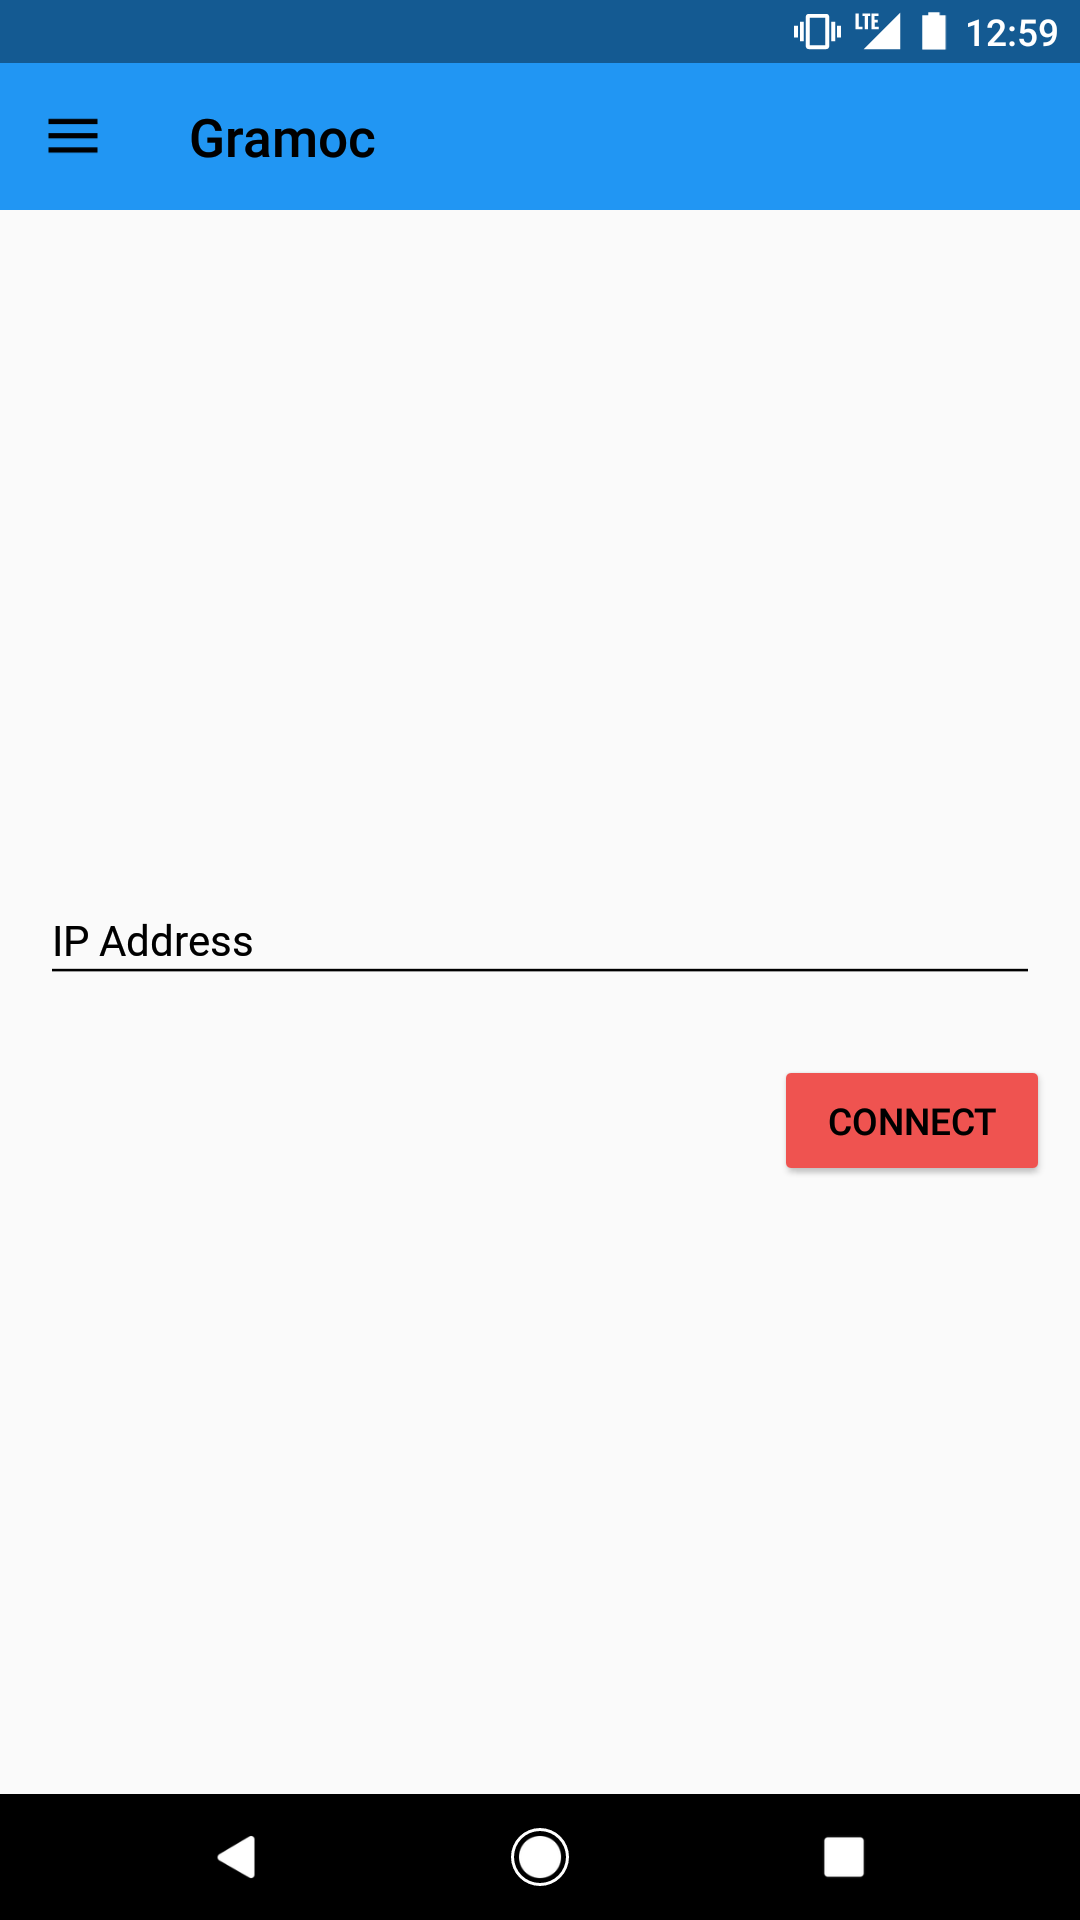
\includegraphics[height=7cm,keepaspectratio]{app_connect}
	&
	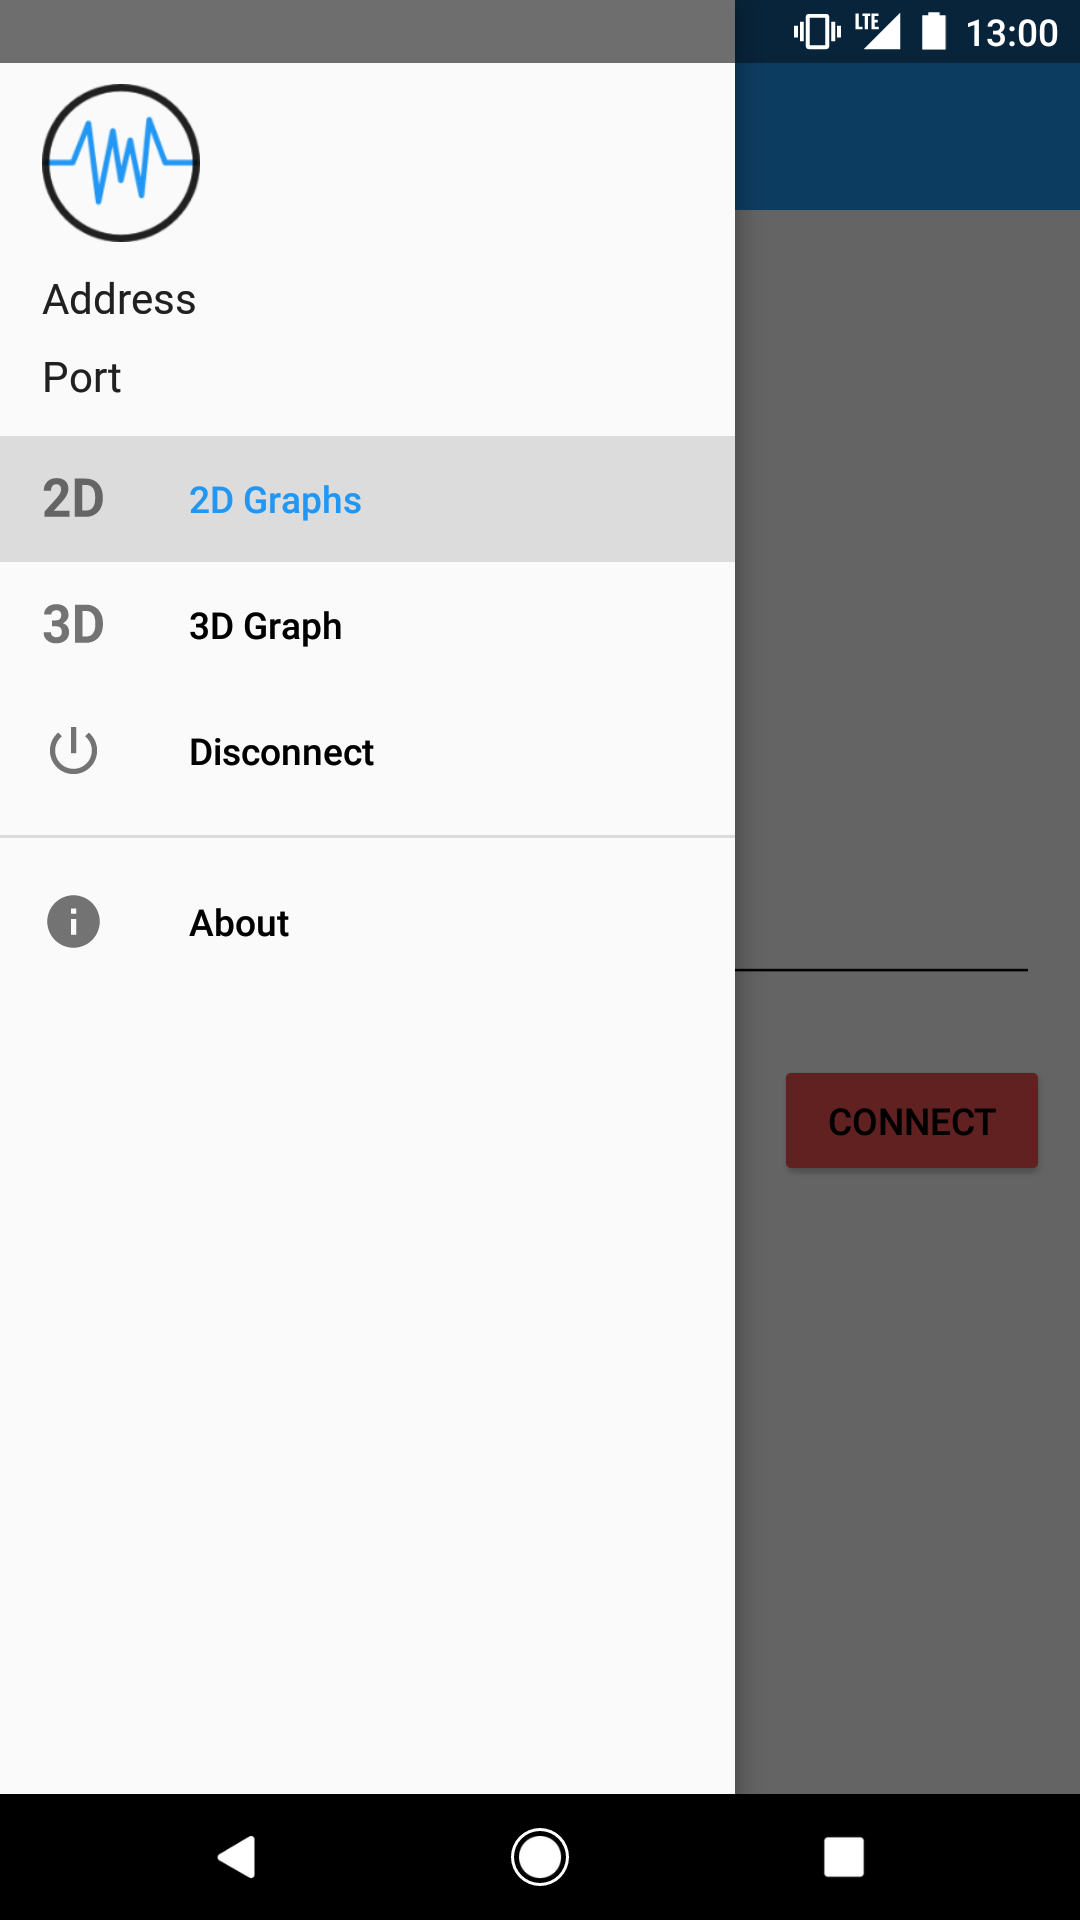
\includegraphics[height=7cm,keepaspectratio]{app_navdrawer}
	\\
	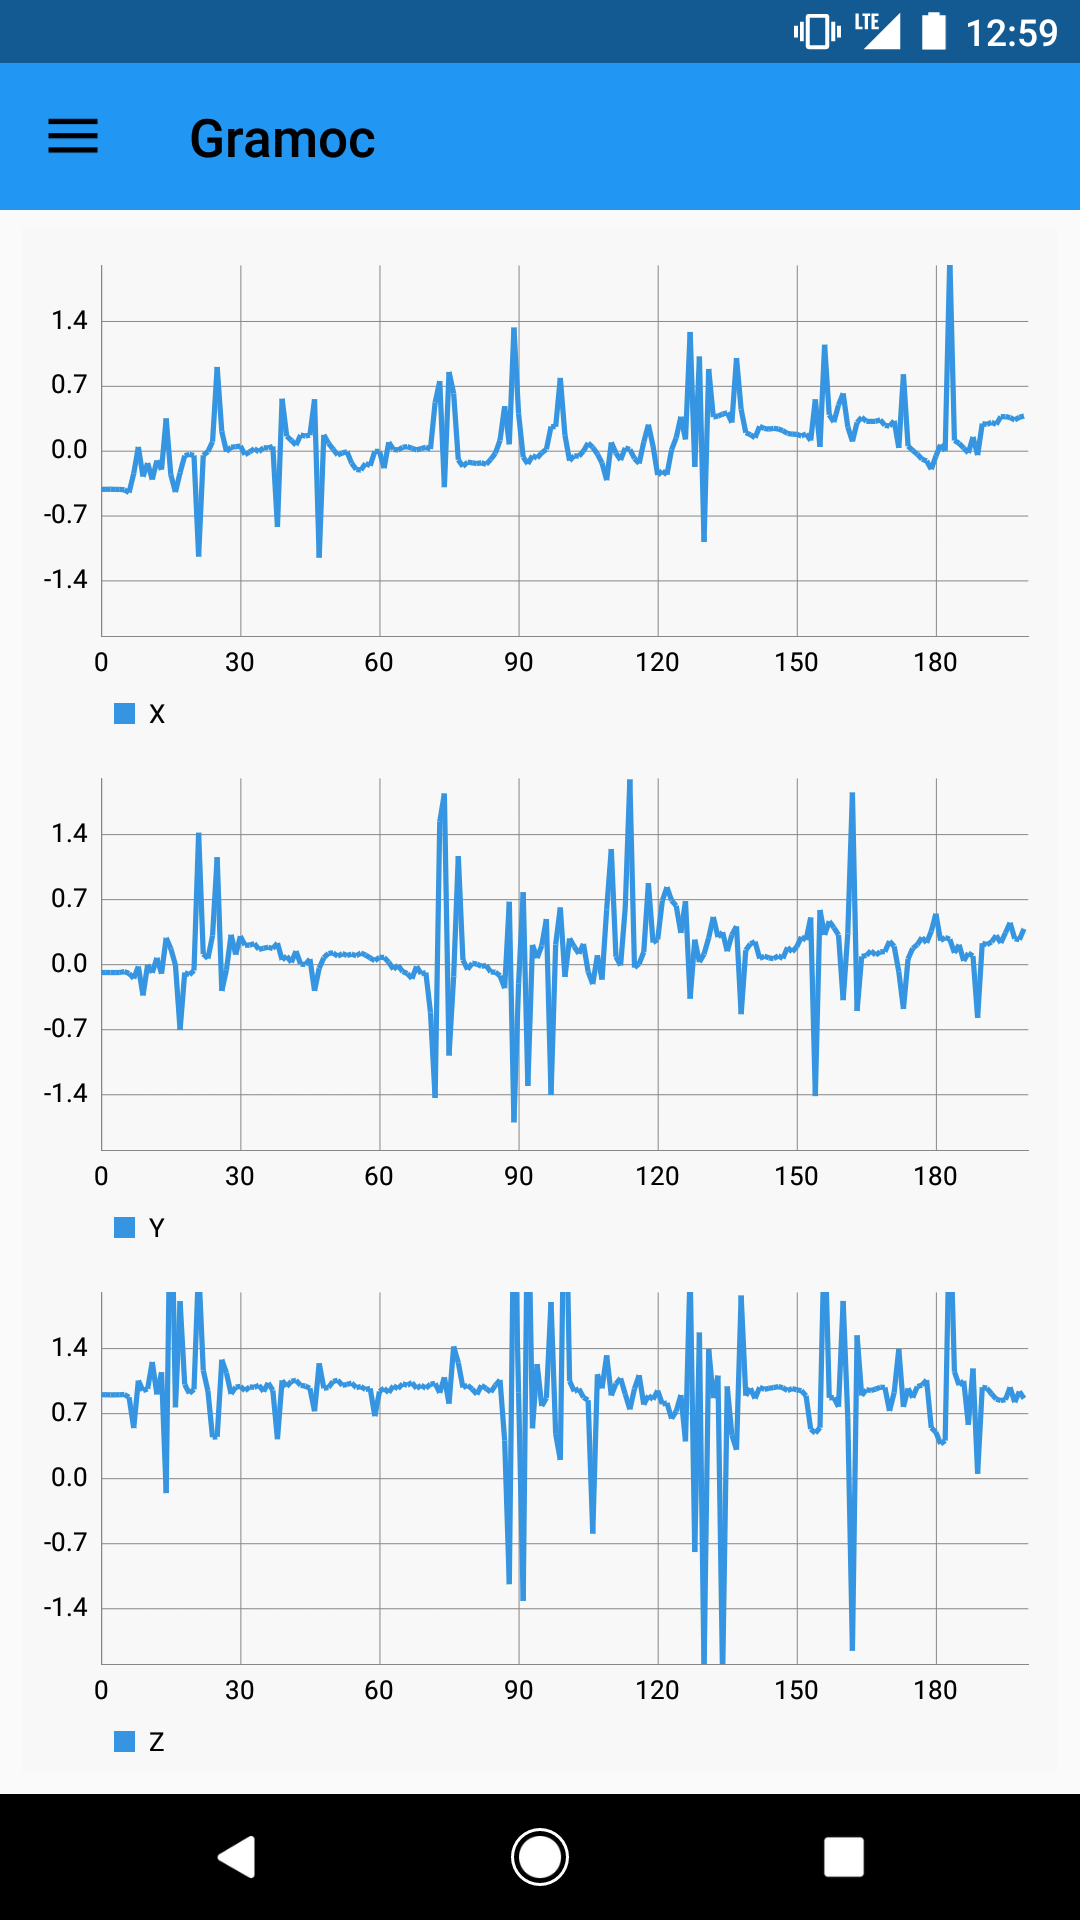
\includegraphics[height=7cm,keepaspectratio]{app_sensor}
	&
	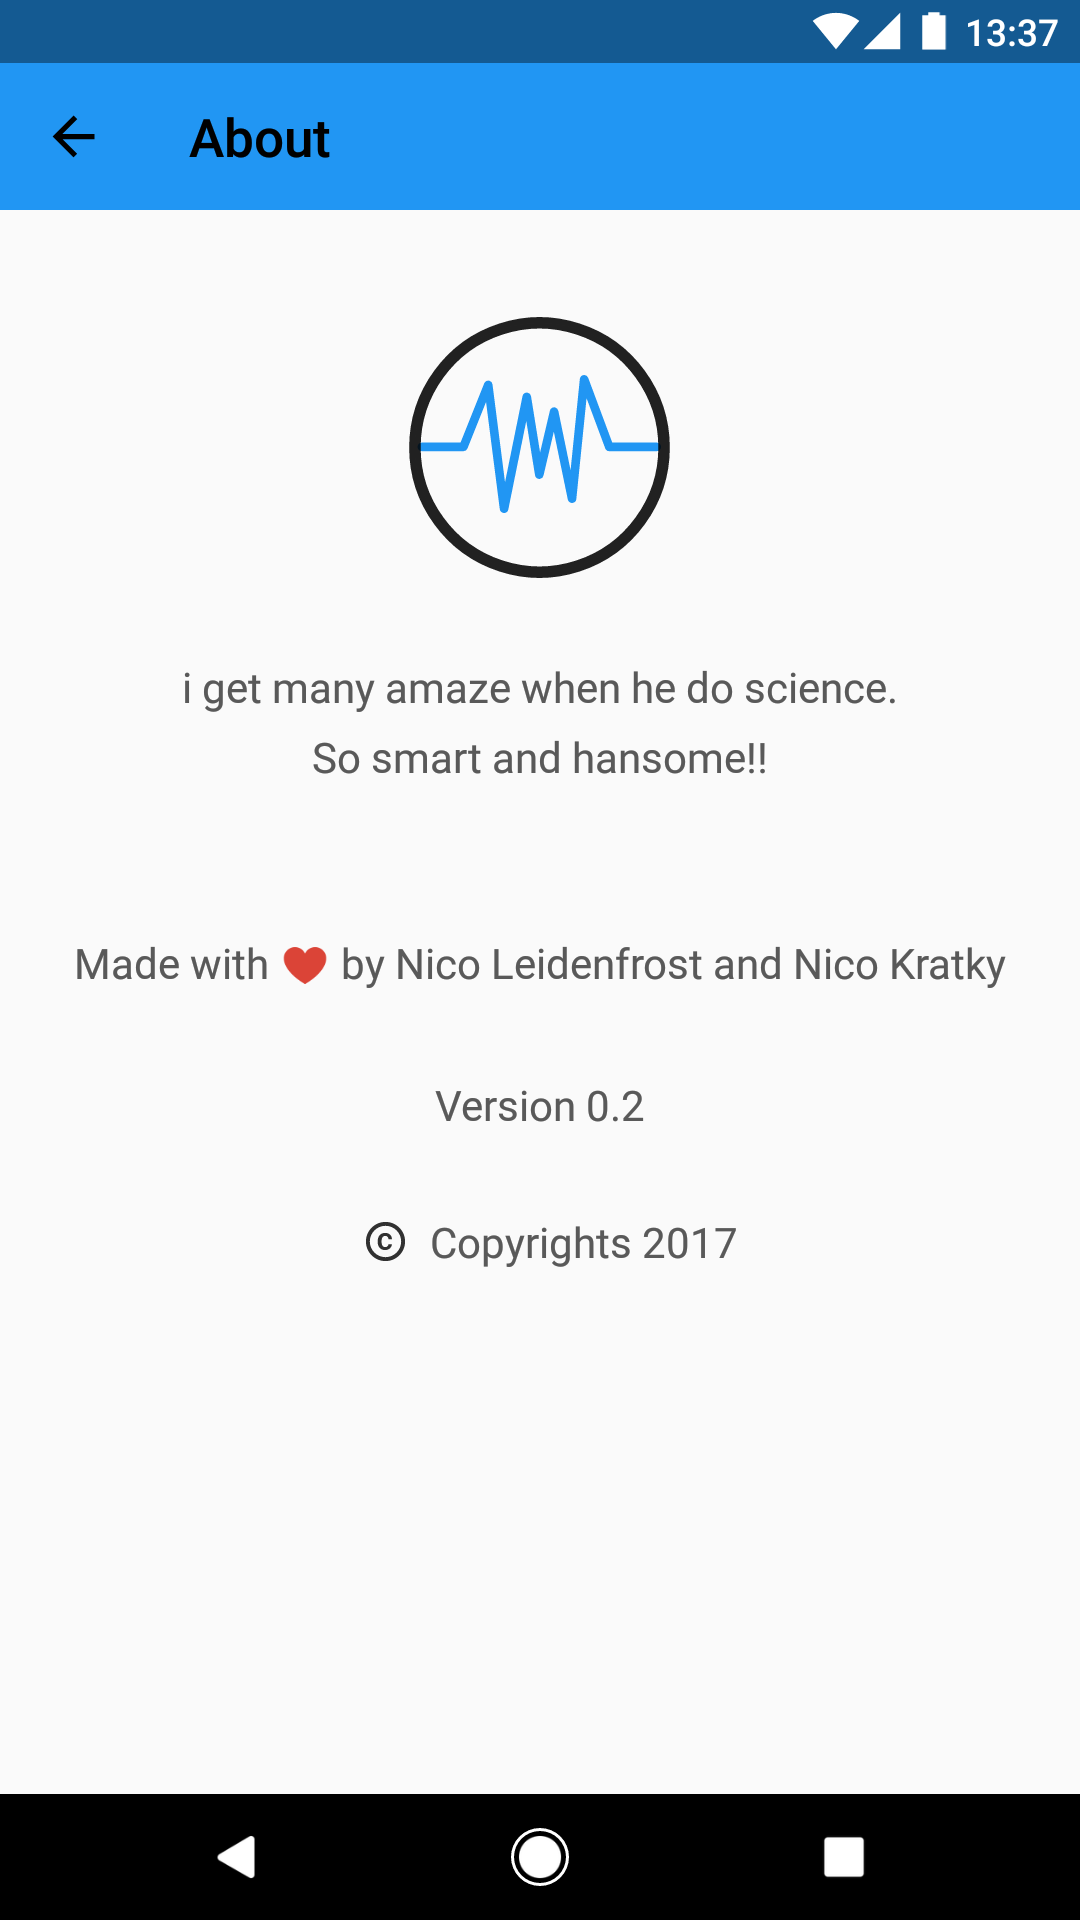
\includegraphics[height=7cm,keepaspectratio]{app_about}
	\end{tabular}
	\caption{Screenshots of App}
	\label{fig:appscreenshots}
\end{figure}

\section{Implementation}
